\chapter{Analiza wyników}

    W niniejszym rozdziale zweryfikowano eksperymentalnie działanie algorytmu EdgeSketch oraz porównano go z algorytmem NodeSketch. Przeprowadzono szereg testów na różnych grafach i zbadano wpływ parametrów na jakość uzyskiwanych wyników. Sprawdzono także średnią liczbę operacji wykonywanych przez algorytmy w zależności od liczby krawędzi w grafie.

\section{Architektura eksperymentów}

    Na działanie algorytmów NodeSketch i EdgeSketch wpływ mają trzy główne parametry. Są to:
    \begin{itemize}
        \item $k$ - rząd sąsiedztwa. Przyjmujemy, że przy $k = 2$ rozpatrujemy tylko bezpośrednie połączenia, przy $k = 3$ także ścieżki długości $2$ itd. 
        \item $m$ - rozmiar szkicu. Jest to liczba elementów w wektorze opisującym pojedynczy wierzchołek w grafie. 
        \item $\alpha$ - parametr rozkładu wykładniczego. Decyduje on, jakie wagi nadawane są sąsiedztwom wyższych rzędów.
    \end{itemize}

    Jednak uzyskiwane wyniki zależą też w naturalny sposób od grafu, na którym przeprowadzane są eksperymenty. W związku z tym, w celu zbadania wpływu tych parametrów na jakość uzyskiwanych wyników, przeprowadzono szereg eksperymentów na różnych grafach. Główną badaną statystyką była precyzja, czyli stosunek liczby poprawnie odgadniętych krawędzi do wartości $t$, a więc wielkości próbki. Rozważano próbki wielkości $t \in \{100, 1000, 10000, |E|\}$, gdzie $|E|$ to liczba krawędzi w grafie. Algorytmy zostały zaimplementowane w języku Julia\cite{Julia}.

\section{Badanie uzyskiwanych wyników w zależności od struktury grafów}

    \subsubsection{Model Erdosa-Renyiego}
        Model Erdosa-Renyiego jest jednym z najpowszechniejszych modeli grafów losowych. W modelu tym, każda para wierzchołków jest połączona krawędzią z jednakowym prawdopodobieństwem $p$. Steruje on gęstością grafu, a co za tym idzie, średnim stopniem wierzchołków. Grafy w tym modelu charakteryzują się dość jednorodną strukturą, bez wyraźnych klastrów, czy wierzchołków o dysproporcjonalnie wysokich stopniach. 

        Eksperyment przeprowadzono dla różnych prawdopodobieństw wystąpienia krawędzi $p$ oraz stopni sąsiedztwa $k \in \{2,3,4\}$. W każdym przypadku liczba wierzchołków w grafie wynosiła $10000$. Rozmiar szkicu wyniósł $m = 10$, a parametr rozkładu wykładniczego $\alpha = 0.3$. Wyniki przedstawiono w tabeli \ref{tab:erdos_renyi}.

        \begin{table}[!ht]
        \small
            \centering
            \begin{tabular}{|l|l|l|l|l|l|l|l|l|l|}
            \hline
                & & \multicolumn{4}{c|}{NodeSketch} & \multicolumn{4}{c|}{EdgeSketch} \\ \cline{1-10}
                \textbf{p} & \textbf{k} & \textbf{t = 100} & \textbf{t = 1000} & \textbf{t = 10000} & \textbf{t = |E|} & \textbf{t = 100} & \textbf{t = 1000} & \textbf{t = 10000} & \textbf{t = |E|} \\ \hline\hline
                \multirow{3}{*}{0.0005} & 2 & 0.94 & 0.762 & 0.4745 & 0.3688 & 1	& 1	& 1	& 0.5562 \\ \cline{2-10}
                & 3 & 0.86 & 0.732 & 0.3947 & 0.2515	& 1	& 1	& 0.9446 &	0.6179 \\ \cline{2-10}
                & 4 & 0.55 & 0.164 & 0.0409 & 0.023	& 1	& 0.985 & 0.8983 & 0.6072 \\ \hline\hline
                \multirow{3}{*}{0.001} & 2 & 0.58 & 0.433 & 0.2779 & 0.2048	& 1	& 1	& 1	& 0.3721 \\ \cline{2-10}
                & 3 & 0.38 & 0.074 & 0.0185 & 0.007	& 1	& 1	& 0.9748 & 0.4285 \\ \cline{2-10}
                & 4 & 0 & 0.004 & 0.0012 & 0.0017 & 1 & 1 & 0.9665 & 0.4301 \\ \hline\hline
                \multirow{3}{*}{0.005} & 2 & 0.26 & 0.144 & 0.0901 & 0.0497	& 1	& 1	& 1	& 0.0981 \\ \cline{2-10}
                & 3 & 0.11 & 0.033	& 0.0137 & 0.0062 & 1 & 0.936 & 0.3025 & 0.0557 \\ \cline{2-10}
                & 4 & 0.01 & 0.006 & 0.0038 & 0.005	& 1	& 0.936	& 0.3025 & 0.0557 \\ \hline\hline
                \multirow{3}{*}{0.01} & 2 & 0.05 & 0.079 & 0.0595 & 0.033	& 1	& 1	& 0.9998 & 0.0576 \\ \cline{2-10}
                & 3 & 0.05 & 0.026 & 0.0157 & 0.0104	& 1	& 1	& 1	& 0.05 \\ \cline{2-10}
                & 4 & 0 & 0.006 & 0.0091 & 0.0102	& 1	& 1	& 1	& 0.05 \\ \hline
            \end{tabular}
            \caption{Model Erdosa-Renyiego}
            \label{tab:erdos_renyi}

        \end{table}

    \subsubsection{Stochastyczny model blokowy}
    Stochastyczny model blokowy (\emph{ang. stochastic block model}) jest modelem, w którym wierzchołki grafu są podzielone losowo na $b$ bloków. Prawdopodobieństwo wystąpienia krawędzi między dwoma wierzchołkami w tym samym bloku wynosi $p$, a pomiędzy wierzchołkami z różnych bloków $q$. Zazwyczaj przyjmuje się $p \gg q$. W modelu tym występują wyraźne klastry, ale stopnie poszczególnych wierzchołków są do siebie dość zbliżone. Sprawdza się on w symulowaniu zbiorów danych, w których można wyróżnić grupy podobnych do siebie punktów, jak np. grupy użytkowników o podobnych zainteresowaniach, albo artykuły z podobnymi słowami kluczowymi. 

    W przeprowadzonym eksprymencie przyjęto rozmiar grafu $n = 1000$, prawdopodobieństwo wystąpienia krawędzi wewnątrz bloku $p = 0.5$ oraz między blokami $q = 0.001$. Zbadano także różne liczby bloków $b \in \{2,4,8\}$. Rozmiar szkicu $m$ ustalono na $10$, a paramter rozkładu wykładniczego wyniósł $\alpha = 0.3$. Wyniki przedstawiono w tabeli \ref{tab:stochastic_block_model}.

    \begin{table}[!ht]
        \small
        \centering
        \begin{tabular}{|l|l|l|l|l|l|l|l|l|l|}
        \hline
            & & \multicolumn{4}{c|}{NodeSketch} & \multicolumn{4}{c|}{EdgeSketch} \\ \cline{1-10}
            \textbf{bloki} & \textbf{k} & \textbf{t = 100} & \textbf{t = 1000} & \textbf{t = 10000} & \textbf{t = |E|} & \textbf{t = 100} & \textbf{t = 1000} & \textbf{t = 10000} & \textbf{t = |E|} \\ \hline\hline
            \multirow{3}{*}{2} & 2 & 0.57 & 0.525 & 0.5136 & 0.5072 & 1 & 1 & 0.4391 & 0.2616 \\ \cline{2-10}
             & 3 & 0.47 & 0.527 & 0.5089 & 0.5016 & 1 & 1 & 0.4545 & 0.3426 \\ \cline{2-10}
             & 4 & 0.44 & 0.523 & 0.5079 & 0.5022 & 1 & 1 & 0.4545 & 0.3426 \\ \hline\hline
            \multirow{3}{*}{4} & 2 & 0.5 & 0.542 & 0.5343 & 0.5131 & 1 & 1 & 0.3352 & 0.1547 \\ \cline{2-10}
             & 3 & 0.53 & 0.483 & 0.4991 & 0.5003 & 1 & 1 & 0.5342 & 0.4087 \\ \cline{2-10}
             & 4 & 0.46 & 0.499 & 0.4983 & 0.5008 & 1 & 1 & 0.5342 & 0.4087 \\ \hline\hline
            \multirow{3}{*}{8} & 2 & 0.66 & 0.594 & 0.5521 & 0.5234 & 1 & 1 & 0.2831 & 0.1289 \\ \cline{2-10}
             & 3 & 0.51 & 0.528 & 0.5158 & 0.5063 & 1 & 0.884 & 0.5825 & 0.4762 \\ \cline{2-10}
             & 4 & 0.5 & 0.496 & 0.5002 & 0.5029 & 1 & 0.884 & 0.5821 & 0.4755 \\ \hline
        \end{tabular}
        \caption{Stochastyczny model blokowy}
        \label{tab:stochastic_block_model}
    \end{table}

    \subsubsection{Model Barabasiego-Alberta}
    W modelu Barabasiego-Alberta (\emph{ang. Barabasi-Albert Model}) wierzchołki dodawane są do grafu sekwencyjnie. Nowy wierzchołek łączy się z istniejącymi wierzchołkami z prawdopodobieństwem proporcjonalnym do ich stopnia. Bardziej formalnie, konstrukcja grafu rozpoczyna się od wyboru małego zbioru $m_0$ początkowycyh wierzchołków i poprowadzenia wśród nich krawędzi w taki sposób, aby każdy wierzchołek był połączony z co najmniej jednym innym. Następnie, w każdym kroku dodawany jest nowy wierzchołek wraz z $m_{ba}$ krawędziami łączącymi go z innymi z prawdopodobieństwem tym większym, im większy jest stopień danego wierzchołka. Konkretnie, prawdopodobieństwo istnienia krawędzi do wierzchołka $i$ wynosi 
    \[
        p_i = \frac{k_i}{\sum_{j \in V^{*}} k_j},
    \]
    gdzie $k_i$ to stopień wierzchołka $i$, a $V^{*}$ to zbiór aktualnie występujących w grafie wierzchołków. W powstałych w ten sposób grafach można zaobserwować duże zróżnicowanie stopni wierzchołków, z wyraźnie odznaczającymi się węzłami centralnymi (\emph{ang. hubs}).

    W przeprowadzonym eksperymencie przyjęto liczbę wierzchołków $n = 1000$ i stopień wierzchołków $m_{ba} \in \{2,4,8\}$, a rozmiar początkowego zbioru wierzchołków ustalono na $m_0 = m_{ba}$. Wyniki przedstawiono w tabeli \ref{tab:barabasi_albert}. W przypadku $m_{ba} = 2$ pominięto wyniki dla $t = 10000$, ponieważ liczba wierzchołków w grafie wynosiła tylko $3994$.
    \begin{table}[!ht]
        \small
        \centering
        \begin{tabular}{|l|l|l|l|l|l|l|l|l|l|}
        \hline
            & & \multicolumn{4}{c|}{NodeSketch} & \multicolumn{4}{c|}{EdgeSketch} \\ \cline{1-10}
            \textbf{m} & \textbf{k} & \textbf{t = 100} & \textbf{t = 1000} & \textbf{t = 10000} & \textbf{t = |E|} & \textbf{t = 100} & \textbf{t = 1000} & \textbf{t = 10000} & \textbf{t = |E|} \\ \hline\hline
            \multirow{3}{*}{2} & 2 & 0.52 & 0.269 & X & 0.2163 & 1 & 0.974 & X & 0.4877 \\ \cline{2-10}
            & 3 & 0.32 & 0.152 & X & 0.1232 & 1 & 0.213 & X & 0.1567 \\ \cline{2-10}
            & 4 & 0.56 & 0.289 & X & 0.2153 & 1 & 0.134 & X & 0.0941 \\ \hline\hline
            \multirow{3}{*}{8} & 2 & 0.19 & 0.14 & 0.0709 & 0.0892 & 1 & 1 & 0.178 & 0.2241 \\ \cline{2-10}
            & 3 & 0.12 & 0.063 & 0.0406 & 0.0511 & 1 & 0.921 & 0.1765 & 0.2222 \\ \cline{2-10}
            & 4 & 0.08 & 0.07 & 0.0313 & 0.0394 & 1 & 0.921 & 0.1765 & 0.2222 \\ \hline\hline
            \multirow{3}{*}{16} & 2 & 0.12 & 0.079 & 0.0939 & 0.0939 & 1 & 1 & 0.2105 & 0.1424 \\ \cline{2-10}
            & 3 & 0.1 & 0.107 & 0.0656 & 0.0595 & 1 & 1 & 0.2197 & 0.1578 \\ \cline{2-10}
            & 4 & 0.06 & 0.028 & 0.0359 & 0.0376 & 1 & 1 & 0.2197 & 0.1578 \\ \hline
        \end{tabular}
        \caption{Model Barabasiego-Alberta}
        \label{tab:barabasi_albert}
    \end{table}

    \subsubsection{Grafy ważone}

    Wyniki dla grafów ważonych przedstawiono w tabeli \ref{tab:weighted_graphs}.

    \begin{table}[!ht]
        \small
        \centering
        \begin{tabular}{|l|l|l|l|l|l|l|l|l|l|}
        \hline
        & & \multicolumn{4}{c|}{NodeSketch} & \multicolumn{4}{c|}{EdgeSketch} \\ \cline{1-10}
                \textbf{p} & \textbf{k} & \textbf{t = 100} & \textbf{t = 1000} & \textbf{t = 10000} & \textbf{t = |E|} & \textbf{t = 100} & \textbf{t = 1000} & \textbf{t = 10000} & \textbf{t = |E|} \\ \hline\hline
            \multirow{3}{*}{0.0005} & 2 & 0 & 0 & 0.0012 & 0.0031 & 1 & 1 & 1 & 0.5505 \\ \cline{2-10}
            & 3 & 0 & 0 & 0.007 & 0.0248 & 1 & 1 & 0.94 & 0.6125 \\ \cline{2-10}
            & 4 & 0 & 0.006 & 0.0122 & 0.012 & 1 & 1 & 0.9207 & 0.6073 \\ \hline\hline
            \multirow{3}{*}{0.001} & 2 & 0 & 0 & 0.0016 & 0.0055 & 1 & 1 & 1 & 0.3721 \\ \cline{2-10}
            & 3 & 0.01 & 0.017 & 0.012 & 0.006 & 1 & 1 & 0.9671 & 0.4235 \\ \cline{2-10}
            & 4 & 0 & 0.003 & 0.0084 & 0.0099 & 1 & 1 & 0.9714 & 0.4275 \\ \hline\hline
            \multirow{3}{*}{0.005} & 2 & 0.01 & 0.008 & 0.0054 & 0.0065 & 1 & 1 & 1 & 0.0989 \\ \cline{2-10}
            & 3 & 0 & 0.007 & 0.0086 & 0.0063 & 1 & 0.941 & 0.3344 & 0.0581 \\ \cline{2-10}
            & 4 & 0 & 0.004 & 0.0064 & 0.0088 & 1 & 0.941 & 0.3344 & 0.0581 \\ \hline\hline
            \multirow{3}{*}{0.01} & 2 & 0 & 0.01 & 0.0086 & 0.0107 & 1 & 1 & 1 & 0.0583 \\ \cline{2-10}
            & 3 & 0.03 & 0.012 & 0.0101 & 0.0117 & 1 & 1 & 1 & 0.05 \\ \cline{2-10}
            & 4 & 0.01 & 0.011 & 0.0151 & 0.0138 & 1 & 1 & 1 & 0.05 \\ \hline
        \end{tabular}
        \caption{Grafy ważone}
        \label{tab:weighted_graphs}
    \end{table}

    \subsection{Wnioski}
    Algorytm EdgeSketch uzyskuje wyższą precyzję niż NodeSketch dla większości zbiorów, na których przeprowadzono eksperymenty. W szczególności dla małych wartości $t$, uzyskiwana przez EdgeSketch precyzja jest bliska $1$, co oznacza że wszystkie lub niemal wszystkie krawędzie zostały przewidziane poprawnie. NodeSketch uzyskuje dość zróżnicowane wyniki, od zbliżonych, lecz nieco niższych, jak w przypadku grafu w modelu Erdosa-Renyiego z parametrem $p = 0.0005$, po bliskie $0$, jak przy gęstrzych grafach w tym samym modelu. Dla obu algorytmów wyniki pogarszają się wraz ze wzrostem $t$, ale EdgeSketch osiąga nadal lepsze wyniki niż NodeSketch na wszystkich grafach poza tymi w stochastycznym modelu blokowym. 
    
    W przypadku algorytmu NodeSketch, wybór większej wartości parametru $k$ zazwyczaj albo nie zmienia znacząco precyzji albo ją pogarsza, niezależnie od $t$. Inaczej jest w przypadku EdgeSketch, gdzie dobór optymalnego $k$ zależy od konkretnego zbioru oraz wartości $t$. O ile w przypadku małych próbek, np $t = 100$, najlepiej sprawdza się $k = 2$, o tyle dla $t = |E|$, dobór większego $k$ może poprawić wyniki, co widać szczególnie wyraźnie w stochastycznym modelu blokowym oraz w rzadkich grafach w modelu Erdosa-Renyiego. 

    W przypadku grafów ważonych, różnica pomiędzy algorytmami jest szczególnie wyraźna. ExpSketch uzyskuje wyniki bardzo zbliżone do tych osiąganych dla grafów nieważonych o podobnej strukturze. Pozostaje on więc skuteczny w przewidywaniu krawędzi. W przypadku NodeSketcha, wyniki są natomiast znacznie gorsze, często bliskie zeru. Wynikać to może z faktu, że algorytm ten tworzy szkic, w którym przechowywane są indeksy wierzchołków, a nie próbki z rozkładu wykładniczego, jak w przypadku EdgeSketcha.

\section{Wykorzystanie stopnia wierzchołków przy rekonstrukcji}
    Jak wspomniano w rozdziale \ref{sec:weight_sum_estimator}, szkice generowane przez algorytm ExpSketch pozwalają na zdefiniowanie nieobciążonego estymatora sumy wag elementów w strumieniu. W przypadku algorytmu EdgeSketch, ExpSketch jest wywoływany dla pojedynczego wierzchołka, a w strumieniu znajdują się wychodzące z niego krawędzie. Jeśli graf jest nieważony, to suma wag krawędzi jest po prostu stopniem wierzchołka. 
    Przeprowadzono eskperyment mający na celu sprawdzenie, czy ta właściwość może być wykorzystana do poprawy jakości rekonstrukcji. Konkretnie podczas wyboru najbardziej podobnych wierzchołków, śledzono liczbę krawędzi wychodzących z każdego z nich. Jeśli wierzchołek $v$ osiągał swój estymowany stopień, to był on pomijany w dalszym procesie.  
    
    Testy przeprowadzono na trzech zbiorach zawierających rzeczywiste dane. Pierwszy z nich to \emph{HomoSapiens}, zbiór danych zawierający relacje między białkami dla gatunku ludzkiego. \emph{Blogcatalog} to zbiór danych zawierający relacje między blogerami, a \emph{dblp} to fragment zbioru autorów artykułów naukowych, gdzie krawędzie reprezentują współautorstwo. W eksperymencie przyjęto $\alpha = 0.3$ oraz $m = 10$. Wyniki przedstawiono w tabeli \ref{tab:degree}.

    \begin{table}[!ht]
        \small
        \centering
        \begin{tabular}{|l|l|l|l|l|l|l|l|l|l|}
        \hline
        & & \multicolumn{4}{c|}{EdgeSketch} & \multicolumn{4}{c|}{EdgeSketch z oszacowaniem stopnia} \\ \cline{1-10}
            \textbf{zbiór danych} & \textbf{k} & \textbf{t = 100} & \textbf{t = 1000} & \textbf{t = 10000} & \textbf{t = |E|} & \textbf{t = 100} & \textbf{t = 1000} & \textbf{t = 10000} & \textbf{t = |E|} \\ \hline\hline
            \multirow{3}{*}{HomoSapiens} & 2 & 1 & 1 & 0.4459 & 0.1202 & 0.99 & 0.998 & 0.4413 & 0.1669 \\ \cline{2-10}
            & 3 & 1 & 1 & 0.3036 & 0.1153 & 1 & 0.999 & 0.2923 & 0.1576 \\ \cline{2-10}
            & 4 & 1 & 1 & 0.3035 & 0.1163 & 1 & 1 & 0.2921 & 0.1573 \\ \hline\hline
            \multirow{3}{*}{blogcatalog} & 2 & 1 & 1 & 0.7757 & 0.0343 & 1 & 1 & 0.7755 & 0.1943 \\ \cline{2-10}
            & 3 & 1 & 1 & 0.7649 & 0.0377 & 1 & 1 & 0.7647 & 0.1988 \\ \cline{2-10}
            & 4 & 1 & 1 & 0.7649 & 0.0377 & 1 & 1 & 0.7647 & 0.1988 \\ \hline\hline
            \multirow{3}{*}{dblp} & 2 & 1 & 1 & 1 & 0.4453 & 0.99 & 0.994 & 0.9489 & 0.426 \\ \cline{2-10}
            & 3 & 1 & 1 & 0.7684 & 0.3214 & 1 & 0.995 & 0.731 & 0.449 \\ \cline{2-10}
            & 4 & 1 & 1 & 0.6666 & 0.2927 & 1 & 0.997 & 0.6317 & 0.4303 \\ \hline
        \end{tabular}
        \caption{Wyniki z wykorzystaniem stopnia wierzchołków przy rekonstrukcji}
        \label{tab:degree}
    \end{table}

    \subsection{Wnioski}
    Wyniki pokazują, że wykorzystanie stopnia wierzchołków przy rekonstrukcji rzeczywiście może wpływać na poprawę precyzji. Jest to szczególnie widoczne dla $t = |E|$. Choć zazwyczaj różnice nie były duże, to np. w przypadku zbioru \emph{blogcatalog} precyzja wzrosła z niecałych $4\%$ do niemal $20\%$, co jest znaczącą poprawą. Nieco gorzej było w przypadku małych $t$, gdzie nieco lepsze wyniki uzyskał oryginalny algorytm.

\section{Wpływ rozmiaru szkicu na uzyskiwane wyniki}
    Jednym z kluczowych parametrów wpływających na działanie algorytmów NodeSketch i EdgeSketch jest rozmiar szkicu. Wybór odpowiedniej wartości $m$ może nie być oczywisty. Z jednej strony, większy szkic jest w stanie przechować więcej infromacji, lecz z drugiej strony, zwiększa to czas obliczeń oraz ilość używanej pamięci. Poniższe eksperymenty miały na celu werykację wpływu rozmiaru szkicu na uzyskiwane wyniki.

    Pierwszy z nich przeprowadzono na zbiorach danych blogcatalog oraz dblp. W obu przypadkach rozważano różne wartości parametru $m \in \{8, 16, 32, 64, 128, 256\}$. W eksperymencie przyjęto $\alpha = 0.3$ oraz $k = 2$. Wyniki przedstawiono w tabeli \ref{tab:sketch_size}.

    Drugi eksperyment przeprowadzono jedynie dla algorytmu EdgeSketch z tymi samymi parametrami. Został on wykonany na $20$ grafach w stochastycznym modelu blokowym, z których każdy miał $1000$ wierzchołków. Zbadano zmiany precyzji dla $t = 10000$ oraz $t = |E|$ wraz z rozmiarem szkicu. Rezulaty ilustruje wykres \ref{fig:precision_m}.
    \begin{table}[!ht]
        \small
        \centering
        \begin{tabular}{|l|l|l|l|l|l|l|l|}
        \hline
        & & \multicolumn{3}{c|}{NodeSketch} & \multicolumn{3}{c|}{EdgeSketch} \\ \cline{1-8}
                \textbf{zbiór danych} & \textbf{m} & \textbf{t = 1000} & \textbf{t = 10000} & \textbf{t = |E|} & \textbf{t = 1000} & \textbf{t = 10000} & \textbf{t = |E|} \\ \hline\hline
        \multirow{6}{*}{blogcatalog} & 8 & 0.031 & 0.0298 & 0.0277 & 1 & 0.6228 & 0.0298 \\ \cline{2-8}
            & 16 & 0.023 & 0.0276 & 0.0292 & 1 & 0.9998 & 0.0474 \\ \cline{2-8}
            & 32 & 0.009 & 0.0224 & 0.034 & 1 & 0.9998 & 0.0805 \\ \cline{2-8}
            & 64 & 0.016 & 0.0224 & 0.0312 & 1 & 1 & 0.138 \\ \cline{2-8}
            & 128 & 0.01 & 0.0185 & 0.0466 & 1 & 1 & 0.2302 \\ \cline{2-8}
            & 256 & 0.018 & 0.0257 & 0.0406 & 1 & 1 & 0.3609 \\ \hline\hline
        \multirow{6}{*}{dblp} & 8 & 0.996 & 0.8975 & 0.5495 & 1 & 1 & 0.3839 \\ \cline{2-8}
            & 16 & 1 & 0.9381 & 0.5892 & 1 & 1 & 0.5737 \\ \cline{2-8}
            & 32 & 1 & 0.9264 & 0.5974 & 1 & 1 & 0.7481 \\ \cline{2-8}
            & 64 & 1 & 0.9333 & 0.589 & 1 & 1 & 0.87 \\ \cline{2-8}
            & 128 & 1 & 0.9389 & 0.6017 & 1 & 1 & 0.9421 \\ \cline{2-8}
            & 256 & 1 & 0.9415 & 0.6051 & 1 & 1 & 0.9757 \\ \hline
        \end{tabular}
        \caption{Wyniki dla różnych rozmiarów szkicu}
        \label{tab:sketch_size}
    \end{table}

    \begin{figure}[!ht]
        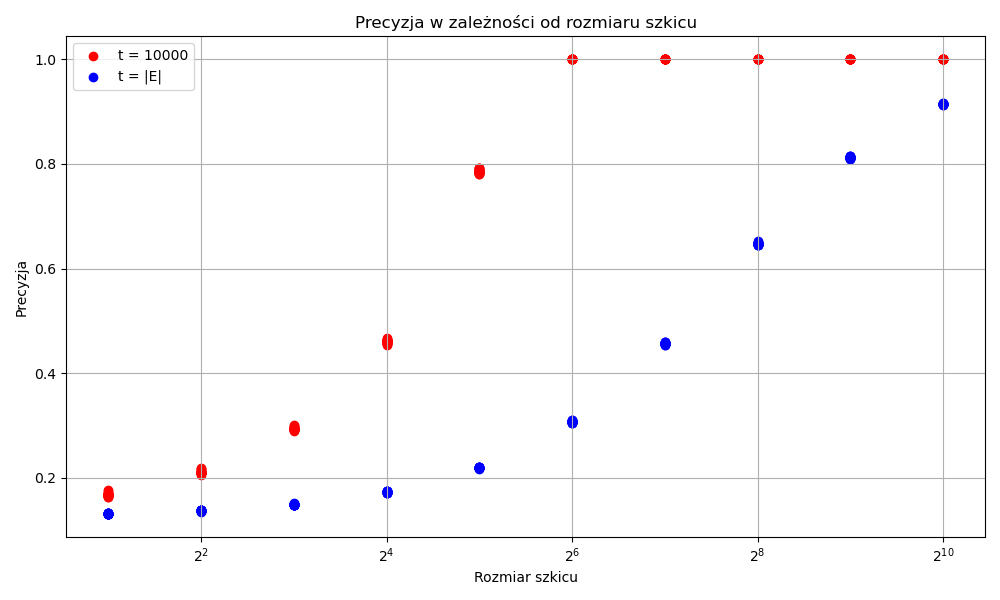
\includegraphics[width=16cm]{img/precision_m.png}
        \centering
        \caption[Precyzja rekonstrukcji]{Precyzja rekonstrukcji w zależności od rozmiaru szkicu dla algorytmu EdgeSketch.}
        \label{fig:precision_m}
    \end{figure}
    
    \subsection{Wnioski}
    Zgodnie z intuicją, zwiększenie rozmiaru szkicu ma korzystny wpływ na uzyskiwaną precyzję. Algorytm EdgeSketch jest szczególnie widoczne w przypadku dużych wartości $t$. Warto jednak zaznaczyć, że im większy szkic, tym dalsze jego zwiększanie ma mniejszy wpływ na precyzję. Co ciekawe, dla małych $t$, EdgeSketch jest w stanie uzyskać wysoką precyzję nawet przy małym rozmiarze szkicu. Przykładowo, dla $t = 10000$, szkic o rozmiarze $64$ jest wystarczający, aby w każdym z badanych przypadków uzyskać precyzję $1$, a w dla zbioru dblp, wystarczający jest nawet szkic o $8$ elementach. W przypadku algorytmu NodeSketch, zyski występują, ale są niewielkie w porównaniu do EdgeSketcha. Warto zaznaczyć, że większy rozmiar szkicu implikuje większą liczbę wykonywanych operacji oraz większe zapotrzebowanie na pamięć, dlatego w praktycznych zastosowaniach konieczne może być znaleznienie kompromisu pomiędzy jakością uzyskiwanych wyników a kosztem obliczeniowym.

\section{Dobór parametru alpha}

    Kolejnym parametrem, mającym znaczenie dla obu algorytmów jest $\alpha$. Jego wartość decyduje, jak szybko maleje wpływ kolejnych, coraz bardziej odległych sąsiadów na generowane szkice, lub, w przypadku EdgeSketcha, obliczane podobieństwa Jaccarda. Grafy wykorzystane w eksperymencie zostały wygenerowane w modelu Erdosa-Renyiego i miały $5000$ wierzchołków. Badano różne wartości $\alpha \in \{0, 0.15, 0.3, 0.45\}$, przy czym $\alpha = 0$ oznacza, że sąsiedztwa wyższych rzędów nie były brane pod uwagę. Rozmiar szkicu $m$ ustalono na $10$, a parametr $k$ na $4$. Rezultaty przedstawiono w tabeli \ref{tab:alpha}.

    \begin{table}[!ht]
        \small
        \centering
        \begin{tabular}{|l|l|l|l|l|l|l|l|l|l|}
        \hline
            & & \multicolumn{4}{c|}{NodeSketch} & \multicolumn{4}{c|}{EdgeSketch} \\ \cline{1-10}
            \textbf{p} & \textbf{$\alpha$} & \textbf{t = 100} & \textbf{t = 1000} & \textbf{t = 10000} & \textbf{t = |E|} & \textbf{t = 100} & \textbf{t = 1000} & \textbf{t = 10000} & \textbf{t = |E|} \\ \hline\hline
        \multirow{4}{*}{0.0005} & 0 & 0.97 & 0.826 & 0.3424 & 0.5415 & 1 & 1 & 0.4462 & 0.7057 \\ \cline{2-10}
            & 0.15 & 0.9 & 0.798 & 0.2917 & 0.4613 & 1 & 1 & 0.4678 & 0.7398 \\ \cline{2-10}
            & 0.3 & 0.95 & 0.782 & 0.2863 & 0.4528 & 1 & 1 & 0.4363 & 0.69 \\ \cline{2-10}
            & 0.45 & 0.9 & 0.788 & 0.2743 & 0.4338 & 1 & 0.785 & 0.3954 & 0.6253 \\ \hline\hline
        \multirow{4}{*}{0.001}    & 0 & 0.91 & 0.69 & 0.4114 & 0.3773 & 1 & 1 & 0.6996 & 0.5548 \\ \cline{2-10}
            & 0.15 & 0.15 & 0.056 & 0.0168 & 0.0146 & 1 & 1 & 0.7469 & 0.6264\\ \cline{2-10}
            & 0.3 & 0.16 & 0.047 & 0.0185 & 0.0164 & 1 & 0.996 & 0.7014 & 0.6161 \\ \cline{2-10}
            & 0.45 & 0.19 & 0.069 & 0.0198 & 0.0173 & 0.97 & 0.939 & 0.6041 & 0.5373 \\ \hline\hline
        \multirow{4}{*}{0.005}    & 0 & 0.38 & 0.258 & 0.144 & 0.0972 & 1 & 1 & 1 & 0.1814 \\ \cline{2-10}
            & 0.15 & 0 & 0.007 & 0.0049 & 0.0053 & 1 & 1 & 0.9276 & 0.1871 \\ \cline{2-10}
            & 0.3 & 0 & 0.004 & 0.0042 & 0.005 & 1 & 0.932 & 0.3196 & 0.1062 \\ \cline{2-10}
            & 0.45 & 0 & 0.006 & 0.0044 & 0.0052 & 0.95 & 0.381 & 0.1227 & 0.0559 \\ \hline\hline
        \multirow{4}{*}{0.01}    & 0 & 0.15 & 0.185 & 0.1091 & 0.0563 & 1 & 1 & 1 & 0.1011 \\ \cline{2-10}
            & 0.15 & 0.01 & 0.011 & 0.0101 & 0.0094 & 1 & 1 & 0.9231 & 0.1022 \\ \cline{2-10}
            & 0.3 & 0.01 & 0.009 & 0.0095 & 0.0095 & 1 & 1 & 0.3234 & 0.0647 \\ \cline{2-10}
            & 0.45 & 0.01 & 0.009 & 0.0094 & 0.0095 & 1 & 0.63 & 0.1928 & 0.0428 \\ \hline
        \end{tabular}
        \caption{Wyniki dla różnych wartości parametru $\alpha$}
        \label{tab:alpha}
    \end{table}

    \subsection{Wnioski}
    Odpowiedni dobór paramtru rozkładu wykładniczego zależy od konkretnego grafu. W badanym modelu dla algorytmu NodeSketch najlepsze wyniki uzyskano ignorując sąsiedztwa wyższych rzędów. Inaczej było w przypadku EdgeSketcha, gdzie niewielkie wartości parametru, zwłaszcza $\alpha = 0.15$ lub $\alpha = 0.3$ wływały korzystnie na uzyskiwane wyniki. Pogarszały się one jednak przy wyborze większych współczynników. Większa $\alpha$ pozwala na ujęcie większej ilości informacji o dalszym sąsiedztwie, ale może również przykrywać informacje o najbliższych sąsiedach wierzchołka, co później zaburza proces rekonstrukcji krawędzi. W większości przypadków wybór małych wartości $\alpha$ wydaje się więc najskuteczniejszą strategią dla algorytmu NodeSketch. 

\section{Liczba operacji w zależności od liczby krawędzi w grafie}
\label{sec:performance}

    Teoretyczna złożoność obliczeniowa algorytmów NodeSketch i EdgeSketch została skomentowana w rozdziale \ref{sec:complexity}. Analiza ta obejmowała wszystkie kroki wykonywane w trakcie działania algorytmów. Jednak w praktyce, pewne operacje mogą mieć o wiele istotniejszy wpływ na ostateczny czas działania niż inne. W szczególności, obliczenie wartości funckji haszujące, choć odbywa się w czasie $O(1)$, to przy dużej liczbie wywołań ma znaczący wpływ na efektywność algorytmu. W poniższym eksperymencie zbadano średnią liczbę obliczonych wartości funkcji haszujących w zależności od liczby krawędzi w grafie. W tym celu wygenerowano grafy w stochastycznym modelu blokowym o różnych rozmiarach, od $200$ do $8000$ wierzchołków. Wszystkie z nich miały $4$ bloki, a prawdopodobieństwa krawędzi wewnątrz bloku i pomiędzy blokami wynosiły odpowiednio $0.5$ i $0.001$. Podobnie jak w innych eksperymentach, rozmiar szkicu $m$ wynosił $10$ i przyjęto $\alpha = 0.3$. Wyniki przedstawiono na wykresie \ref{fig:calculated_hashes_vs_edges_all}. Dodatkowo, wykres \ref{fig:calculated_hashes_vs_edges_relative} przedstawia te same wyniki, ale znormalizowane względem liczby krawędzi w grafie. Warto zaznaczyć, że w implementacji algorytmu NodeSketch zastosowano podobną optymalizację jak w algorytmie EdgeSketch, polegającą na obliczanniu wartośći funkcji haszującej tylko dla niezerowych elementów w macierzy $SLA$. 

\begin{figure}[!ht]
    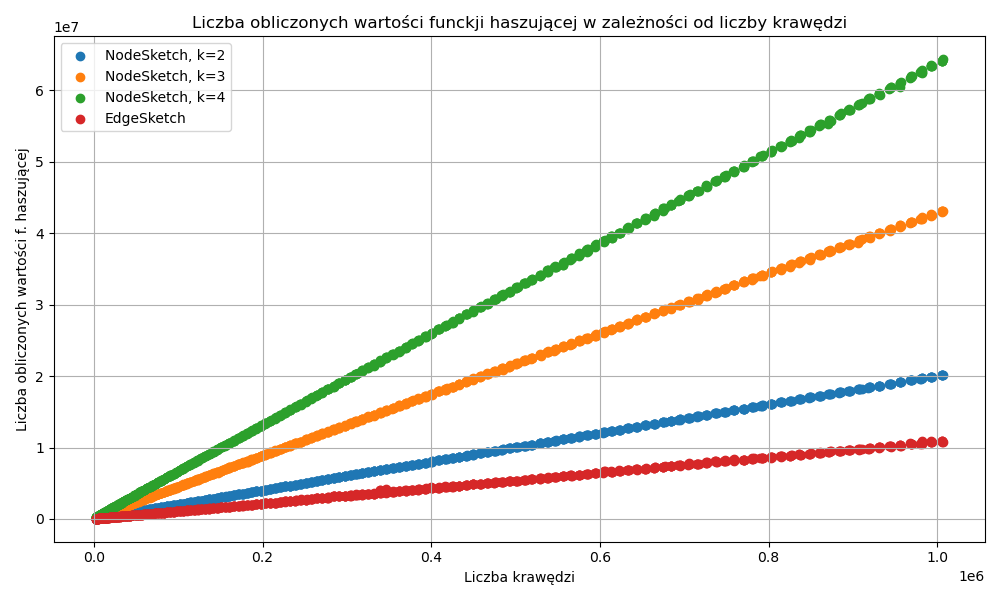
\includegraphics[width=16cm]{img/calculated_hashes_vs_edges_all.png}
    \centering
    \caption[Liczba operacji]{Liczba obliczonych wartości funkcji haszującej w zależności od liczby krawędzi w grafie}
    \label{fig:calculated_hashes_vs_edges_all}
\end{figure}

\begin{figure}[!ht]
    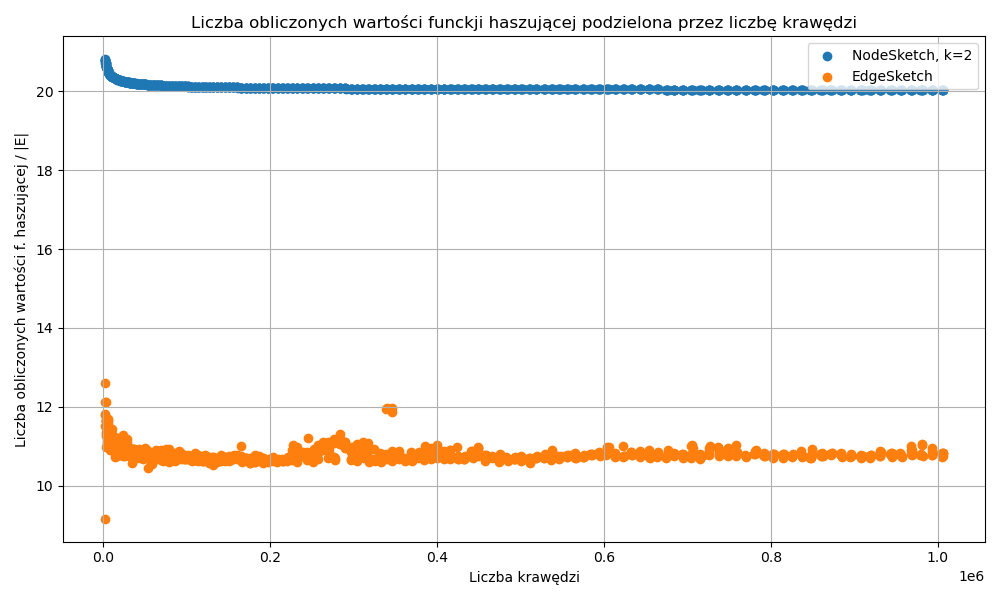
\includegraphics[width=16cm]{img/calculated_hashes_vs_edges_relative.png}
    \centering
    \caption[Liczba operacji znormalizowana]{Liczba obliczonych wartości funkcji haszującej znormalizowana względem liczby krawędzi w grafie}
    \label{fig:calculated_hashes_vs_edges_relative}
\end{figure}

\subsection{Wnioski}
W przypadku obu algorytmów, liczba wywołań funkcji haszującej rośnie liniowo wraz z liczbą krawędzi w grafie. Jest to spodziewany wynik, ponieważ każda krawędź może być wykorzystywana tylko przy generowaniu zanurzeń dla dwóch wierzchołków, które ją wyznaczają. Jest to także zgodne z teoretyczną złożonością obliczeniową algorytmu EdgeSketch. Zauwazyżmy, że procedura FastExpSketch jest wywoływana $|V|$ razy, a średnia liczba przekazywanych do niej elementów to iloraz liczby krawędzi i liczby wierzchołków, a więc gęstość grafu 
\[
    \rho = \frac{|E|}{|V|},
\]
która w rozważanym modelu jest stała. Ostatecznie otrzymujemy więc:
\[
    O(|V| \frac{|E|}{|V|} \ln(\rho)) = O(|E| \ln(\rho)) = O(|E|)
\]

Wraz ze wzrostem parametru $k$, NodeSketch wykonuje więcej operacji ze względu na rekurencyjną procedurę szkicowania. Oczywiście EdgeSketch generuje zanurzenia tylko raz, co daje mu porzewagę przy rozważaniu wyższych stopni sąsiedztwa. Jednak nawet dla $k = 2$, EdgeSketch wykonuje wyraźnie mniej wywołań funckji haszującej niż NodeSketch.

Na drugim wykresie widać ukazującym liczbę wywołań podzieloną przez liczbę krawędzi, widać, że stosunek ten jest rzeczywiście liniowy. Jedynie dla małych grafów odznaczają się nieco większe wartości. Wynika to z faktu, że algorytmy wykorzystują macierz $SLA$, a nie zwykłą macierz sąsiedztwa, a więc biorą pod uwagę sztuczną pętle od wierzchołka do siebie samego, nie ujętą w zaprezentowanej liczbie krawędzi. Dla algorytmu NodeSketch stosunek ten stabilizuję się na ok $20$. Wynika to z faktu, że szkic ma rozmiar $10$, a każdą z krawędzi rozważamy dla dokładnie dwóch wierzchołków. Wykorzystanie procedury FastExpSketch pozwala zredukować tę wartość prawie dwukrotnie, choć jest to okupione większą wariancją.  
